% Name: Generative adversarial network
% Description: A generator that turns noise into fake samples and a discriminator that tells them from real data, each trained against the other.
% Tags: GAN, generator, discriminator, generative model

\usetikzlibrary{arrows.meta, positioning}

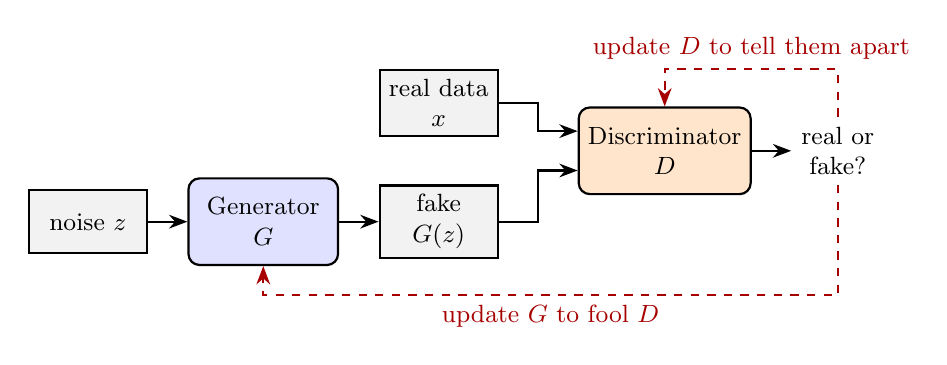
\begin{tikzpicture}[>={Stealth}, thick, node distance=5mm, every node/.style={font=\small},
    net/.style={draw, rounded corners, minimum width=19mm, minimum height=11mm, align=center},
    data/.style={draw, fill=gray!10, minimum width=15mm, minimum height=8mm, align=center}]
  \node[data] (z) {noise $z$};
  \node[net, fill=blue!12, right=of z] (G) {Generator\\$G$};
  \node[data, right=of G] (fake) {fake\\$G(z)$};
  \node[data, above=6mm of fake] (real) {real data\\$x$};
  \node[net, fill=orange!20, right=10mm of fake, yshift=9mm] (D) {Discriminator\\$D$};
  \node[right=of D, align=center] (out) {real or\\fake?};
  \draw[->] (z) -- (G);
  \draw[->] (G) -- (fake);
  \draw[->] (fake.east) -- ++(5mm,0) |- ([yshift=-2.5mm]D.west);
  \draw[->] (real.east) -- ++(5mm,0) |- ([yshift=2.5mm]D.west);
  \draw[->] (D) -- (out);
  % Both networks learn from the discriminator's verdict.
  \draw[->, dashed, red!65!black] (out.south) |- ++(0,-1.4) -| node[pos=0.25, below] {update $G$ to fool $D$} (G.south);
  \draw[->, dashed, red!65!black] (out.north) |- ++(0,0.6) -| node[pos=0.25, above] {update $D$ to tell them apart} (D.north);
\end{tikzpicture}
